\subsection{Jointly Localizing and Describing Events for Dense Video Captioning}

\subsubsection{Overview}

\par Yehao Li \textit{et al}, in their 2018 paper titled \textit{Jointly Localizing and Describing Events for Dense Video Captioning} \cite{li2018jointly}, proposed descriptiveness regression for dense video captioning in end-to-end manner. The network is inspired from the architecture of object localization network \cite{ren2016faster}. The sentence-generation also employs a policy-gradient based reinforcement learning method to optimize LSTM with evaluation metric based reward.


\subsubsection{Datasets}
\begin{itemize}
\item ActivityNet Captions
\end{itemize}

\subsubsection{Performance}
\par Li \textit{et al} compared captioning results with LSTM \cite{venugopalan2015translating}, S2VT \cite{venugopalan2015sequence}, H-RNN \cite{yu2016video}, Temporal Attention \cite{yao2015describing} and DCE \cite{krishna2017densecaptioning} using BLEU@1-4, METEOR and CIDEr. The model performed better with both ground-truth and learnt proposals. 


\subsubsection{Methodology}

\par Li \textit{et al} architecture consists of two main components:
\begin{enumerate}
	\item Temporal Event Proposal(TEP) Module
	\item Sentence Generation (SG) Module
\end{enumerate}

\begin{figure}[h]
	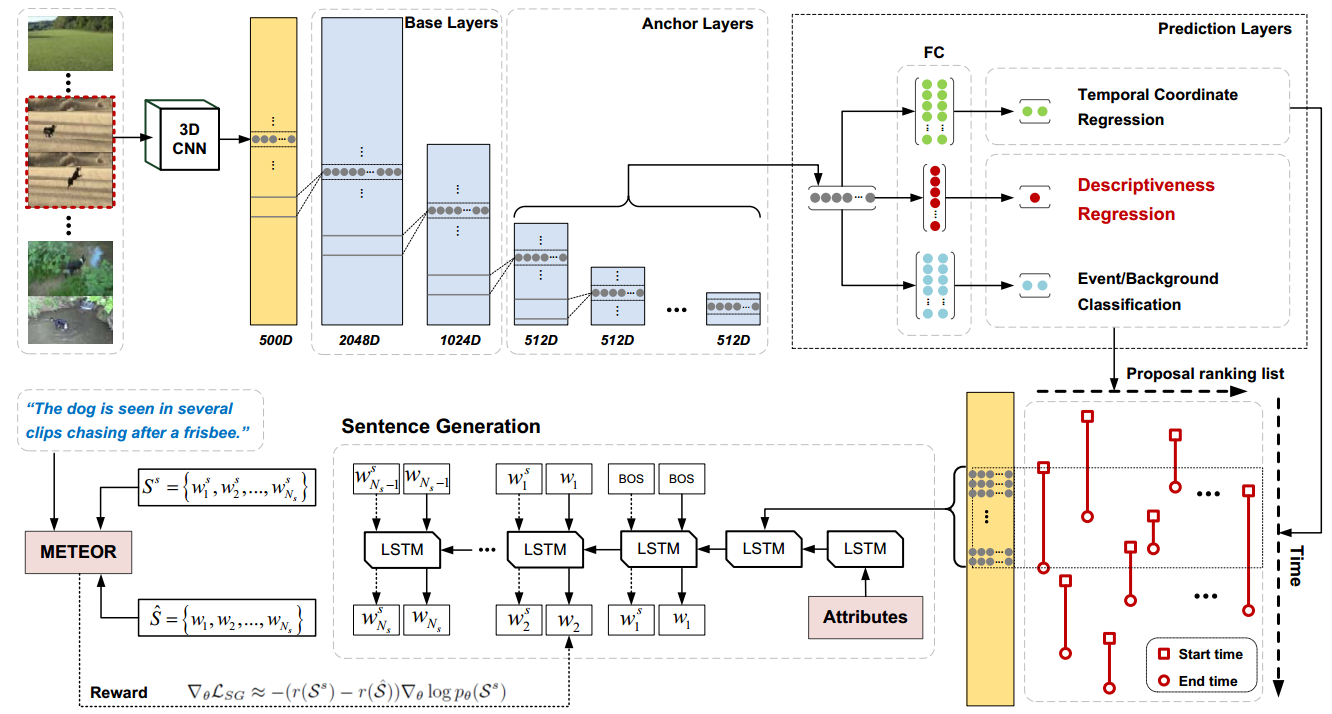
\includegraphics[width=\linewidth]{assets/img/li2018jointly-architecture.png}
	\caption{Architecture introduced by Li \textit{et al} (Image courtesy \cite{li2018jointly})}
\end{figure}

\paragraph{Temporal Event Proposal(TEP) Module} - Generate Candidate proposals
\begin{enumerate}
	\item \textit{Input}: Video frames.
	\item Encode video frames using 3D-CNN and pass it to 1D-CNN architecture, Base layers, anchor layers and prediction layer.
	\item \textit{Output}: $\{t_{start}, t_{end}, p_{event}, p_{des}\}_1^{N_p}$
	\begin{enumerate}
		\item $N_p$: Total number of candidate proposals.
		\item $p_{event}$: probability of recognizing the candidate as an event (i.e., eventness score). 2D vector - [$p_{event}$, $p_{background}$].
		\item $p_{des}$: descriptiveness score measuring how well the candidate can be described from language perspective.
	\end{enumerate}
	\item Rank proposals based on $p_{conf} = p_{event} + \lambda_0p_{des}$
\end{enumerate}

\paragraph{Sentence Generation (SG) Module} - Generate captions for final proposals
\begin{enumerate}
	\item \textit{Input}:
	\begin{enumerate}
		\item A - Attributes from 200 categories of ActivityNet dataset
		\item F - Encoded representation of frames in that proposal (weighted attention using descriptiveness score)
	\end{enumerate}
	\item Each proposal is injected into attribute-augmented LSTM. Firstly the attributes representation A of predicted proposal is transformed into LSTM to inform the whole LSTM about the high-level attributes, followed by the proposal representation F which is encoded into LSTM at the second time step.
	\item LSTM decodes each output word based on previous word and previous step’s LSTM hidden state.
	\item Inspired from reinforcement learning, LSTM is optimized using minimizing the expected sentence-level reward loss.
	\item \textit{Output}: Sentence describing that proposal.
\end{enumerate}


\subsubsection{Conclusion}

\par Li \textit{et al} introduced the concept of descriptiveness regression in dense video captioning to make the process end-to-end. The model is able to adjust the
event proposal from language perspective in TEP module and measure the descriptive complexity of each event in SG module.